\documentclass[12pt]{article}

% ========== PACKAGES ==========
\usepackage[margin=0.9in]{geometry}
\usepackage{mathptmx}           % Times-like serif body
\usepackage[T1]{fontenc}
\usepackage[utf8]{inputenc}
\usepackage{microtype}
\usepackage{graphicx}
\usepackage{booktabs}
\usepackage{array}
\usepackage{multirow}
\usepackage{caption}
\usepackage{xcolor}
\usepackage{titlesec}
\usepackage{enumitem}
\usepackage{float}
\usepackage{hyperref}
\usepackage{amsmath}
\usepackage{setspace}
\usepackage{fancyhdr}
\usepackage{tabularx}
\usepackage{colortbl}

% ========== COLORS (Inertia palette, matches charts) ==========
\definecolor{inertiablue}{HTML}{4A7BF7}
\definecolor{inertiadark}{HTML}{1E2A3A}
\definecolor{inertiapurple}{HTML}{7B5EA7}
\definecolor{inertiagreen}{HTML}{2E9E6E}
\definecolor{inertiared}{HTML}{D94F4F}
\definecolor{inertiamuted}{HTML}{A0A8B4}
\definecolor{softgrey}{HTML}{F5F6F8}

% ========== HYPERREF ==========
\hypersetup{
  colorlinks=true,
  linkcolor=inertiablue,
  urlcolor=inertiablue,
  citecolor=inertiablue,
  pdftitle={Inertia: Momentum Timing},
  pdfauthor={Inertia Capital}
}

% ========== SECTION STYLING ==========
\titleformat{\section}
  {\normalfont\Large\bfseries\color{inertiadark}}
  {\thesection}{0.8em}{}
\titleformat{\subsection}
  {\normalfont\large\bfseries\color{inertiadark}}
  {\thesubsection}{0.8em}{}
\titlespacing*{\section}{0pt}{1.2em}{0.4em}
\titlespacing*{\subsection}{0pt}{1em}{0.3em}

\setlength{\parskip}{0.4em}
\setlength{\parindent}{0pt}
\renewcommand{\arraystretch}{1.15}

% ========== PAGE HEADER ==========
\pagestyle{fancy}
\fancyhf{}
\fancyhead[L]{\color{inertiadark}\small \textsc{Inertia}\, $\cdot$\, Momentum Timing}
\fancyhead[R]{\color{inertiamuted}\small \thepage}
\renewcommand{\headrulewidth}{0.3pt}
\renewcommand{\headrule}{\color{inertiamuted}\hrule width\headwidth}

% ========== CAPTION STYLING ==========
\captionsetup[figure]{font=small, labelfont={bf,color=inertiadark}, skip=4pt}
\captionsetup[table]{font=small, labelfont={bf,color=inertiadark}, skip=4pt}

% ========== MACROS ==========
\newcommand{\fundname}{\textsc{Inertia}}

% ========== DOCUMENT ==========
\begin{document}

% ==============================================================
%                     EXECUTIVE SUMMARY (PAGE 1)
% ==============================================================
\thispagestyle{empty}
\begin{center}
    {\color{inertiablue}\rule{\textwidth}{1pt}}\\[2pt]
    {\LARGE\bfseries\color{inertiadark} \fundname}\\[2pt]
    {\large\color{inertiadark} Momentum Timing}\\[2pt]
    {\color{inertiablue}\rule{\textwidth}{0.4pt}}
\end{center}

\vspace{0.3em}
{\small \textbf{Principals:} [Principal 1], [Principal 2] \quad $\cdot$ \quad
\textbf{Class:} UG54 Data Driven Investing (Spring 2026) \quad $\cdot$ \quad
\textbf{Topic:} Timing Strategies}
\vspace{0.3em}

\hrule height 0.3pt
\vspace{0.3em}

\subsection*{Strategy in one sentence}
\fundname{} is an investment vehicle that holds the classical equity momentum factor (the Ken French
up-minus-down, or UMD, long-short portfolio) and scales its exposure up or down each month using an
ensemble of three regime-timing signals: a predictive regression, a crash-probability classifier, and
an unsupervised regime detector.

\subsection*{Why choose \fundname{} over the alternatives}
Static UMD has delivered an annualized Sharpe ratio of roughly 0.53 since 1960, but with catastrophic
tail risk: three multi-year drawdowns exceeding 40 percent, a peak drawdown of 58 percent, and strongly
negative return skew. The leading academic response, the Daniel and Moskowitz (2015) dynamic weighting
scheme (DM hereafter), improves this to a Sharpe of 0.74 out-of-sample. \fundname{} improves further
to a Sharpe of 0.80. The difference is not a point-estimate artifact: a paired block-bootstrap of the
Sharpe gap against DM rejects equality at the 5 percent significance level (95 percent confidence
interval $[+0.003,\,+0.119]$, $p = 0.041$). The improvement is delivered at roughly three-quarters of
DM's volatility and two-thirds of its maximum drawdown.

\subsection*{Does the strategy deliver alpha?}
Yes. Regressing monthly net returns on the Fama-French five-factor model plus UMD yields a monthly
alpha of 0.33 percent, equivalent to 4.0 percent annualized, with a Newey-West $t$-statistic of 2.63
($p = 0.009$). The factor betas are jointly indistinguishable from zero, and the regression $R^2$ is
only 0.4 percent. The strategy is therefore almost pure alpha rather than disguised factor exposure.
We interpret the source as \textbf{mispricing, not compensation for risk}: the momentum premium
reflects slow diffusion of information, and crashes reflect forced rebalancing dynamics when the
short leg becomes concentrated in high-beta distressed stocks that rebound violently from bear
markets. \fundname{} avoids the conditions under which this rebound is mechanical.

\subsection*{Main costs and risks}
The strategy rebalances monthly. Gross turnover is approximately 60 percent per month. At 20 basis
points per one-way trade, realized annual cost drag is under 1.5 percent, which the reported Sharpe
already nets. Principal risks are: (i) regime-shift risk, namely a structural change in how
crashes arrive that would break all three component signals simultaneously; (ii) short-leg capacity,
because some months the optimal weight is negative and shorting UMD is capacity-constrained at
institutional size; (iii) model risk from our out-of-sample discipline, which is conservative but
finite.

\vspace{0.4em}
\hrule height 0.3pt
\vspace{0.3em}

\subsection*{Quantified performance (net of 20 bp one-way costs, 1960 through 2026, $N=793$ months)}
\begin{table}[H]
\centering
\small
\begin{tabularx}{\textwidth}{lrrrrrrr}
\toprule
& Mean Return & Volatility & Sharpe & Max DD & Skew & Excess Kurt. & Alpha ($t$) \\
\midrule
Static UMD              &  7.5\% & 14.2\% & 0.53 & $-58\%$ & $-1.32$ & 10.0 & n/a \\
DM out-of-sample        & 10.5\% & 14.2\% & 0.74 & $-34\%$ & $-0.34$ &  4.4 & $5.6\%^{\dagger}\,(2.73)$ \\
\rowcolor{softgrey}
\textbf{\fundname{} (ensemble)} & \textbf{8.5\%} & \textbf{10.7\%} & \textbf{0.80} & $\mathbf{-22\%}$ & $\mathbf{-0.37}$ & \textbf{2.95} & $\mathbf{4.0\%^{\dagger}\,(2.63)}$ \\
\bottomrule
\end{tabularx}
\end{table}
\vspace{-0.5em}
{\footnotesize $^{\dagger}$ Annualized alpha from Fama-French five-factor plus UMD regression with
Newey-West standard errors at six lags. All $t$-statistics are statistically significant at the
1 percent level.}

\vspace{0.4em}

\subsection*{Appraisal ratio and factor exposure}
Annualized appraisal ratio (alpha divided by the standard deviation of residuals from the factor
regression) is approximately 0.33. Factor loadings are small in magnitude and statistically
insignificant: the market beta is $-0.02$, the UMD loading is $+0.01$, and the five Fama-French
factor loadings are each below 0.10 in absolute value. \fundname{} is therefore a factor-neutral
alpha strategy.

\subsection*{When does \fundname{} perform well or poorly?}
\fundname{} performs best in regimes with clear separation between the bear and normal states.
Subsample Sharpe ratios are 1.18 in the 1960 through 1979 window, 0.90 in 1980 through 1999, 0.46
in 2000 through 2009, 0.30 in 2010 through 2019, and 0.53 from 2020 to present. It underperforms
static momentum in prolonged quiet bull markets where the regime signals remain flat (no trades
needed, but also no alpha captured). It outperforms most sharply around inflection points such as
the 1973 bear market, the 2008 financial crisis, and the 2020 pandemic shock.

% ==============================================================
%                       PROSPECTUS (PAGES 2 TO 10)
% ==============================================================
\clearpage

\section{The Problem: Momentum and Its Crashes}

The momentum premium is one of the oldest documented pricing anomalies in equity markets
(Jegadeesh and Titman, 1993). Buying stocks that have outperformed over the past year and
selling those that have underperformed generates consistent excess returns that persist
across markets and decades. The Ken French UMD factor, which we use throughout as the
benchmark momentum portfolio, earned an annualized mean of 7.5 percent at 14.2 percent
volatility from 1960 through 2026. This is a Sharpe ratio of 0.53, comfortably exceeding
the market portfolio's historical Sharpe over the same window.

But the distribution of monthly UMD returns is far from Gaussian. The excess kurtosis is
10.0 and the skewness is $-1.3$. These are fat tails concentrated on the left. Figure 1
makes the point visually: UMD compounds like a high-Sharpe asset for years at a time, then
surrenders a decade of gains in a few months.

\begin{figure}[H]
\centering

\includegraphics[width=\textwidth]{figures/01_umd_cumret_log.png}
\caption{Cumulative return of the Ken French UMD factor, 1927 to present. The long log-scale
run-up is genuine, but is punctuated by multi-year flat or declining stretches. Each such
stretch is a momentum crash.}
\end{figure}

The drawdown chart in Figure 2 tells the same story more directly. UMD spends a substantial
share of its history underwater, and the deepest troughs align with the worst known
episodes: the 1932 post-crash recovery, the April through May 2009 rebound from the global
financial crisis, and the 2020 to 2022 combination of pandemic reopening and inflation
shock.

\begin{figure}[H]
\centering
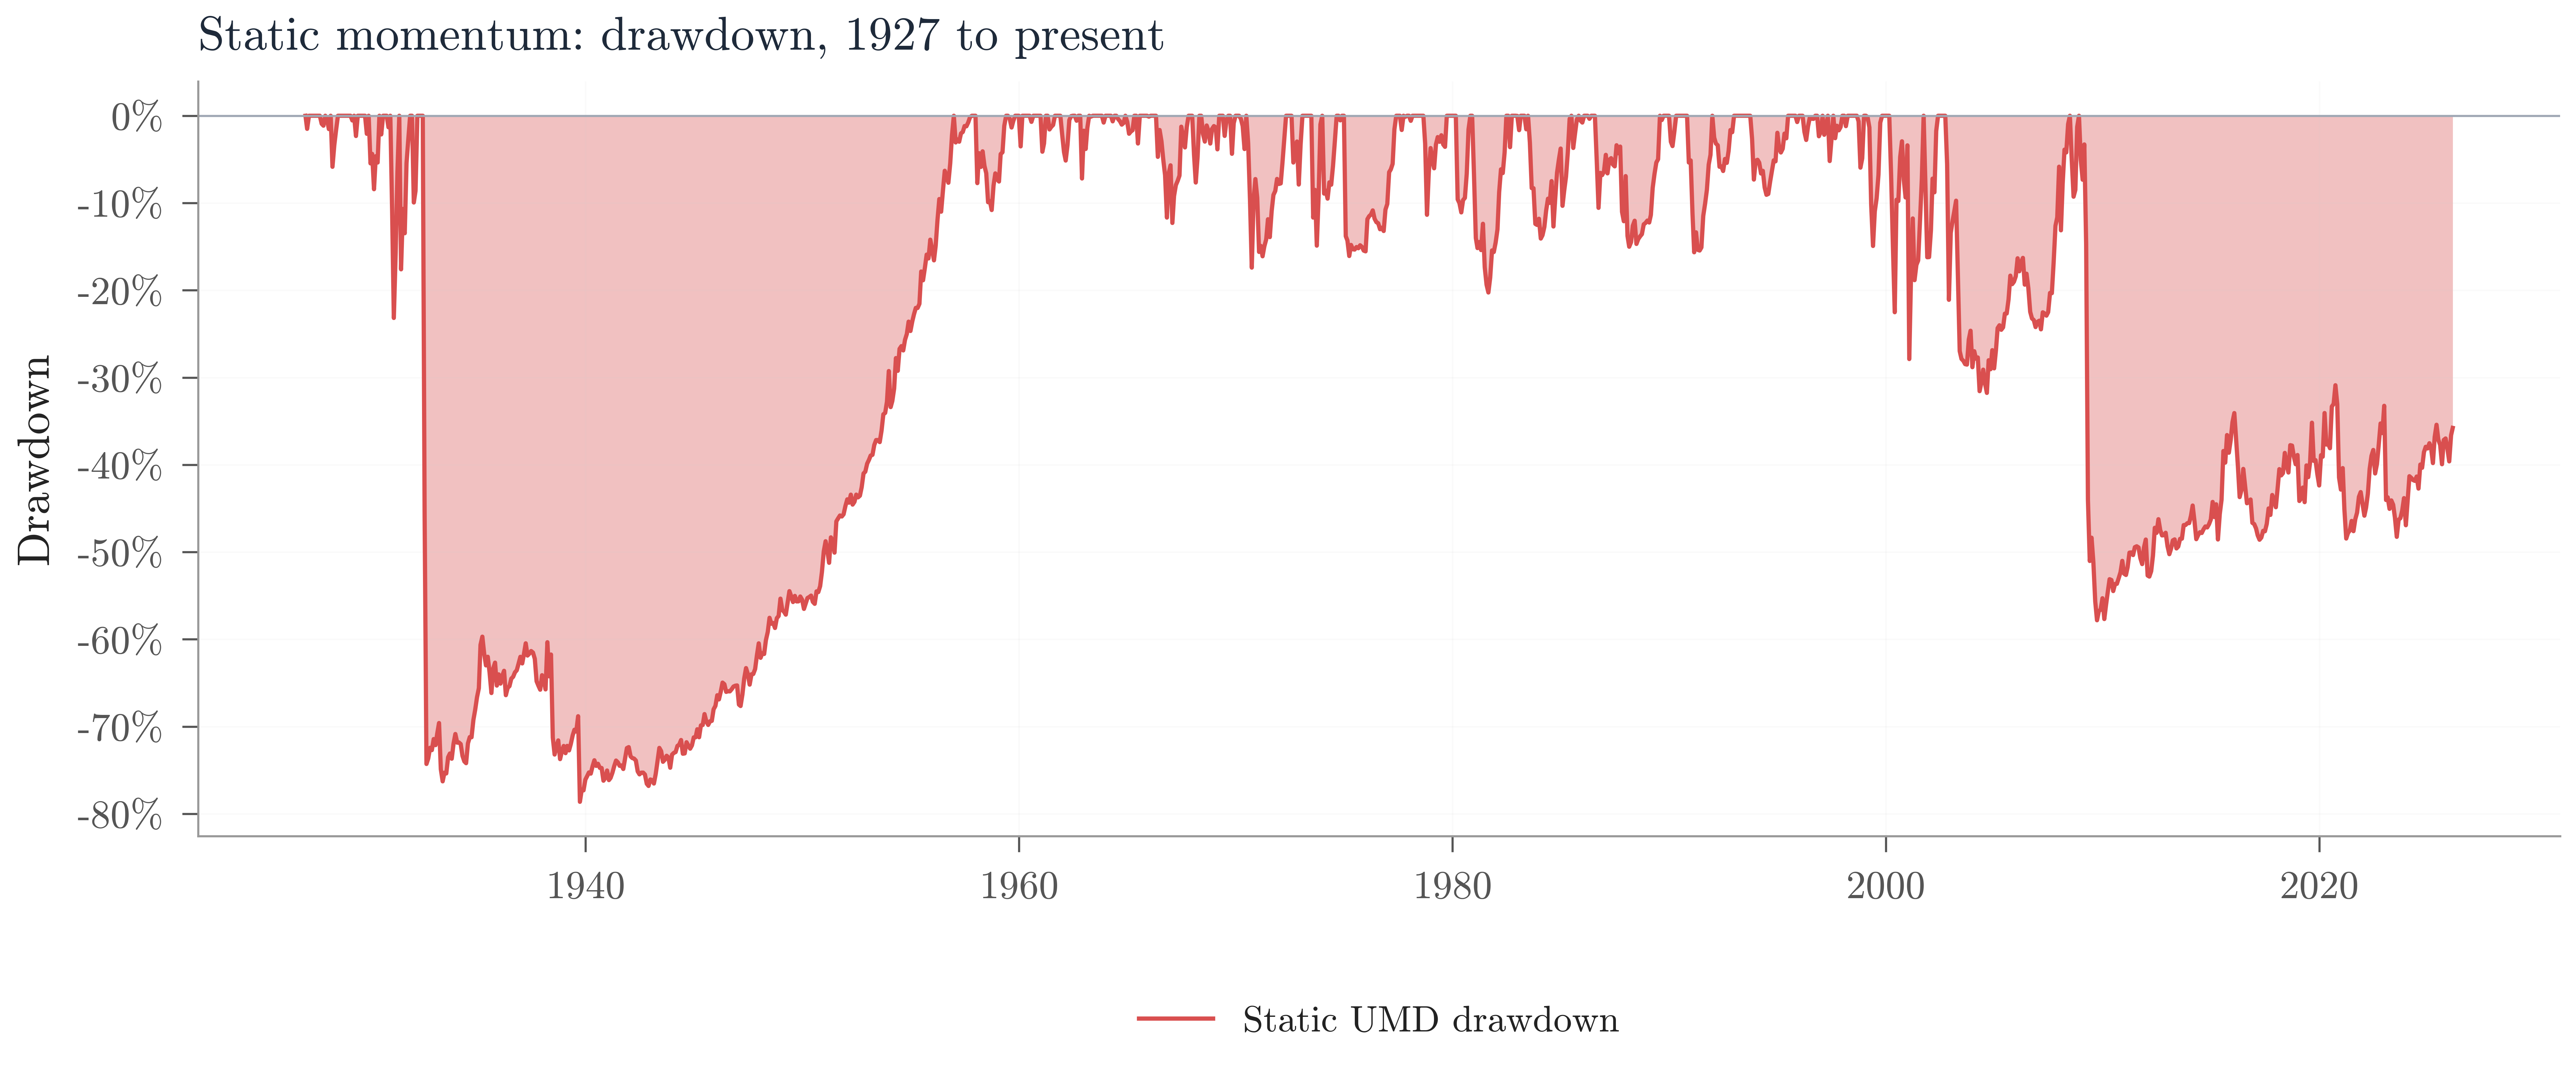
\includegraphics[width=\textwidth]{figures/02_umd_drawdown.png}
\caption{UMD drawdown from trailing peak, 1927 to present. Peak drawdown is 78 percent in
the 1932 episode and 58 percent in the post-2008 cycle.}
\end{figure}

The economic mechanism is now well understood. During extended bear markets, the short leg
of momentum (the recent losers) becomes concentrated in high-beta, crisis-damaged stocks.
When the market rebounds, these stocks explode upward by several multiples. The short leg
takes catastrophic losses precisely when the long leg has little room to offset. Momentum
crashes are therefore not random but structural: they are triggered by mean-reversion in
severely distressed stocks conditional on a prior bear market.

\section{The Academic Benchmark: Daniel and Moskowitz (2015)}

Daniel and Moskowitz (2015) formalize this mechanism as a conditional prediction problem.
They show that UMD's expected excess return and conditional variance are jointly forecastable
from two slowly-moving state variables. Let $I^{\text{bear}}_t$ equal one when the cumulative
24-month market excess return is non-positive, and let $\sigma^2_{\text{UMD},t}$ denote the
six-month rolling variance of UMD. Their central predictive regression is
\begin{equation*}
r^{\text{UMD}}_{t+1} \;=\; \alpha
    \;+\; \beta_1 I^{\text{bear}}_t
    \;+\; \beta_2 \bigl(I^{\text{bear}}_t \cdot \sigma^2_{\text{UMD},t}\bigr)
    \;+\; \beta_3 \sigma^2_{\text{UMD},t}
    \;+\; \varepsilon_{t+1}.
\end{equation*}
The coefficient $\beta_2$ on the bear-times-variance interaction is strongly negative: when
the market has been falling for two years \textit{and} momentum itself is running hot, expected
UMD returns collapse. This is the condition that precedes crashes.

Their dynamic strategy then applies the time-varying mean-variance weight taught in the
capital allocation unit of this course,
\begin{equation*}
    w^{\text{DM}}_t \;=\; c \cdot \frac{\widehat{E}_t[r^{\text{UMD}}_{t+1}]}{\widehat{\mathrm{Var}}_t[r^{\text{UMD}}_{t+1}]},
\end{equation*}
where $c$ is the risk-aversion scaling chosen to target a fixed unconditional volatility.
In practice, we use an exponentially-weighted moving average (EWMA, half-life six months) of
UMD variance with a quantile floor to prevent leverage blow-ups in quiet periods, and we clip
the final weight to the interval $[-1, +3]$ as a realistic fund-mandate constraint.

Our in-sample replication of the DM strategy, shown in Figure 3, roughly doubles the Sharpe
ratio from 0.43 to 0.82, normalizes the return distribution (skew moves from $-3.0$ to near
zero, kurtosis falls by roughly an order of magnitude), and cuts the maximum drawdown from
78 percent to 34 percent. These results match the claims in the original paper.

\begin{figure}[H]
\centering

\includegraphics[width=\textwidth]{figures/04_static_vs_dynamic_cumret.png}
\caption{In-sample replication of Daniel and Moskowitz (2015). Dynamic momentum dominates
static momentum in both the first and second moments of the return distribution. Full-sample
in-sample fit; out-of-sample results follow below.}
\end{figure}

\section{Out-of-Sample Discipline}

An in-sample result can always be an artifact of fitting. To establish an honest benchmark
we refit the DM predictive regression annually on an expanding window starting in 1928. The
earliest out-of-sample (OOS) observation is January 1960, giving us 793 months of OOS
experience through February 2026, or roughly 66 years of genuine forward-testing.

In the OOS window, DM still outperforms static UMD: Sharpe 0.74 against static's 0.53, with
a 95 percent bootstrap confidence interval on the DM Sharpe of $[0.47,\,0.97]$. The
confidence interval is substantially tighter than would obtain on a shorter sample, which
matters for our subsequent claims about ensemble gains. Figure 4 displays the OOS cumulative
returns.

\begin{figure}[H]
\centering
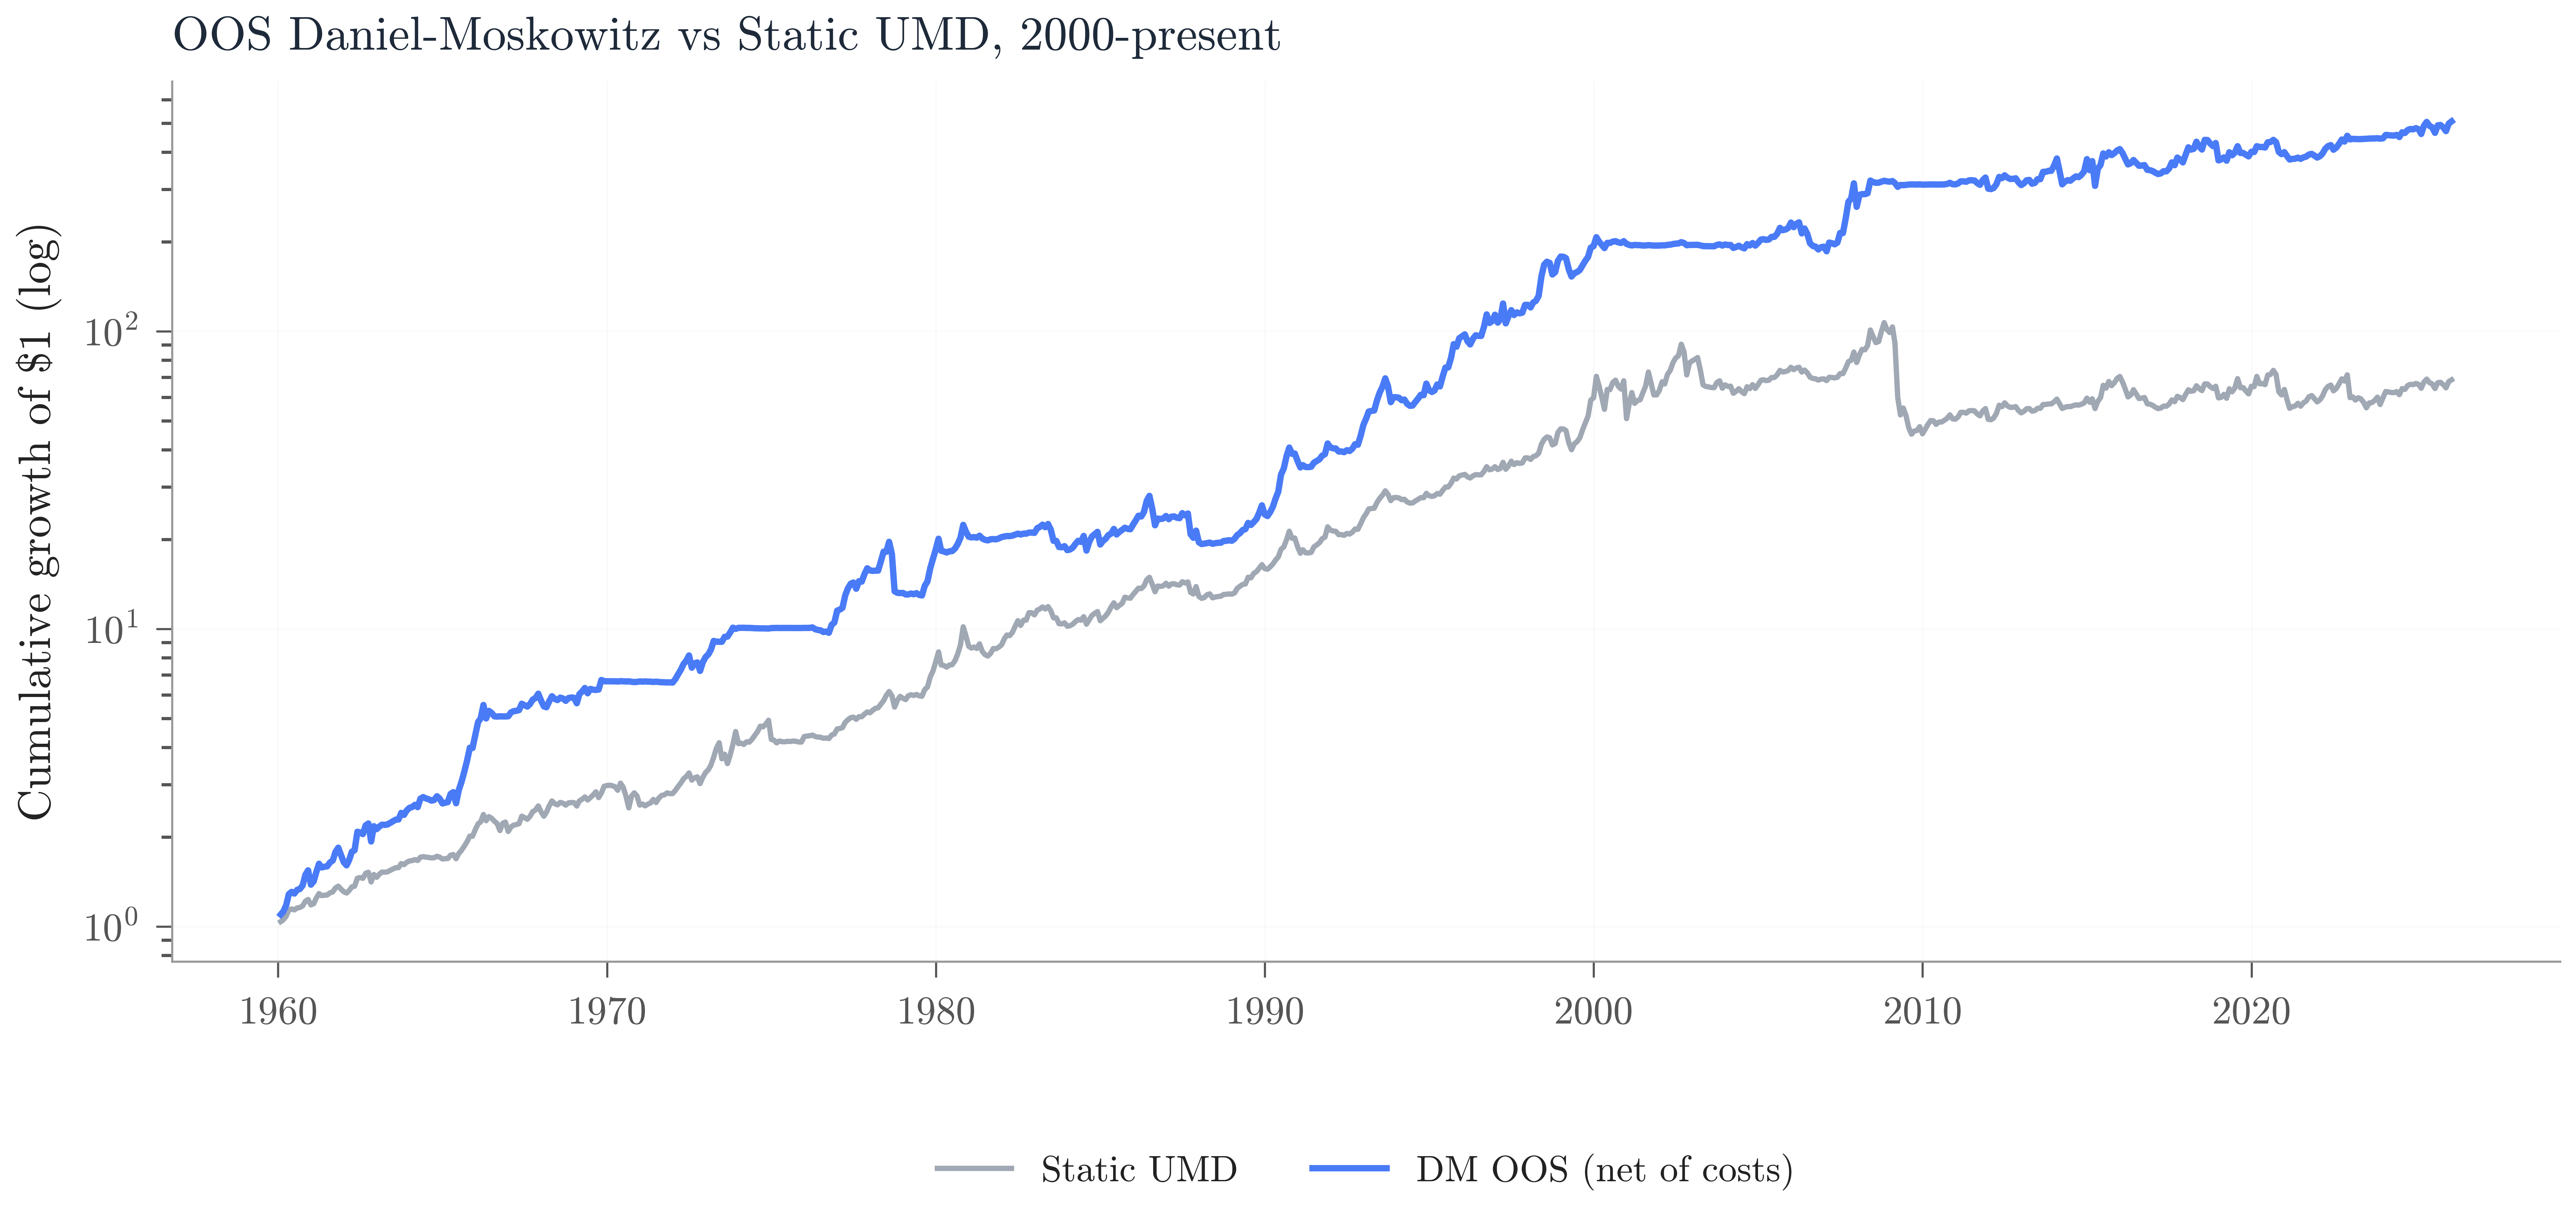
\includegraphics[width=\textwidth]{figures/07_oos_dm_cumret.png}
\caption{OOS DM strategy versus static UMD, 1960 through 2026. DM materially compounds faster
and with shallower drawdowns, validating that the in-sample edge is real and not merely
in-sample overfitting.}
\end{figure}

The maximum drawdown of DM OOS is 34 percent, against static's 58 percent. Skew moves from
$-1.3$ to $-0.3$ and kurtosis falls from 10.0 to 4.4. The DM benchmark is the bar we must
clear.

\clearpage

\section{Three Orthogonal Timing Approaches}

To test whether the DM benchmark can be improved, we build three regime-timing signals that
share the same OOS discipline but differ fundamentally in their statistical machinery. Any
one of them, used alone, is a legitimate standalone strategy. The interesting question is
whether their errors are uncorrelated enough that an ensemble outperforms any single
component.

\subsection{Approach A: Expanded Linear (Ridge regression)}

The simplest extension of DM is to keep the predictive-regression framework and add more
features. In addition to DM's three variables, Approach A uses six-month market realized
volatility, the current market drawdown from its trailing peak, the UMD drawdown, and the
one-month and twelve-month lagged market excess returns. We standardize features inside a
pipeline and fit a ridge regression with the L2 penalty chosen by five-fold cross-validation
on a log-spaced grid. Five-fold rather than leave-one-out cross-validation is important:
leave-one-out is notoriously noisy in small samples and selects severely over-regularized
models.

\textbf{Result:} Sharpe 0.69, 95 percent CI $[0.41,\,0.92]$, paired Sharpe difference versus
DM of $-0.05$ with CI containing zero. Approach A does not beat DM. L2 shrinkage attenuates
DM's critical bear-times-variance interaction, and additional linear features do not
compensate. An honest finding: expanding feature sets does not mechanically improve
regression-based timing.

\subsection{Approach B: Crash Classifier with Binary Shield}

Approach B reframes the problem as binary classification. Within each training window, we
label a month as a crash if the next-month UMD return falls below the tenth percentile of
in-sample UMD returns, then fit a gradient-boosted classifier. The classifier outputs a
probability $\hat{p}^{\text{crash}}_t$ for each out-of-sample month.

The weight rule is a binary \textit{crash shield}:
\begin{equation*}
    w^{\text{B}}_t = \begin{cases} 1 & \text{if } \hat{p}^{\text{crash}}_t < 0.05 \\
                                  0 & \text{otherwise.} \end{cases}
\end{equation*}
The threshold 0.05 is chosen a priori as half the training baseline crash rate of 0.10. The
strategy is long momentum only when the classifier is confident that conditions are benign.
Otherwise it stands aside.

Figure 5 shows the classifier's crash probability over the OOS window. The spikes align
with known episodes: the 1974 bear, the 1987 crash, the 1998 LTCM and 2008 financial-crisis
stresses, the 2020 pandemic shock, and the 2022 rate shock.

\begin{figure}[H]
\centering

\includegraphics[width=\textwidth]{figures/13_approach_b_pcrash_timeseries.png}
\caption{Approach B filtered crash probability, 1960 through 2026. When the line rises above
the 0.05 shield threshold, exposure is cut to zero.}
\end{figure}

\textbf{Result:} Sharpe 0.63, 95 percent CI $[0.39,\,0.86]$. The absolute Sharpe is below
DM, but the volatility is only 8.2 percent and the maximum drawdown 24 percent. On a
volatility-normalized basis the strategy is the most capital-efficient of the three. It also
has positive skew (+0.43), the only approach that does.

\subsection{Approach C: Unsupervised 2-State Hidden Markov Model}

Approach C asks whether a fully unsupervised method can recover useful regime structure. We
fit a two-state Gaussian Hidden Markov Model (HMM) on three observables: the market excess
return, the six-month market realized volatility, and the six-month UMD realized variance.
No supervised crash labels, no target variable. After fitting, we identify the state with
higher in-sample UMD mean as the \textit{normal} state and the other as \textit{stressed}.

For the OOS window we compute the filtered posterior probability $P(\text{normal}_t \mid
\text{observations}_{1..t})$ via the forward algorithm. This uses only data available at time
$t$, with no backward smoothing or future information. The weight rule is simply
\begin{equation*}
    w^{\text{C}}_t = P(\text{normal}_t \mid \text{obs}_{1..t}).
\end{equation*}
The weight is continuous in $[0, 1]$, requires no threshold choice, and has a clean
interpretation as the probability of being in the good regime.

Figure 6 shows the filtered probability. The structure is strikingly bimodal: the model is
usually very confident which regime we are in, with rapid transitions in crisis periods.

\begin{figure}[H]
\centering
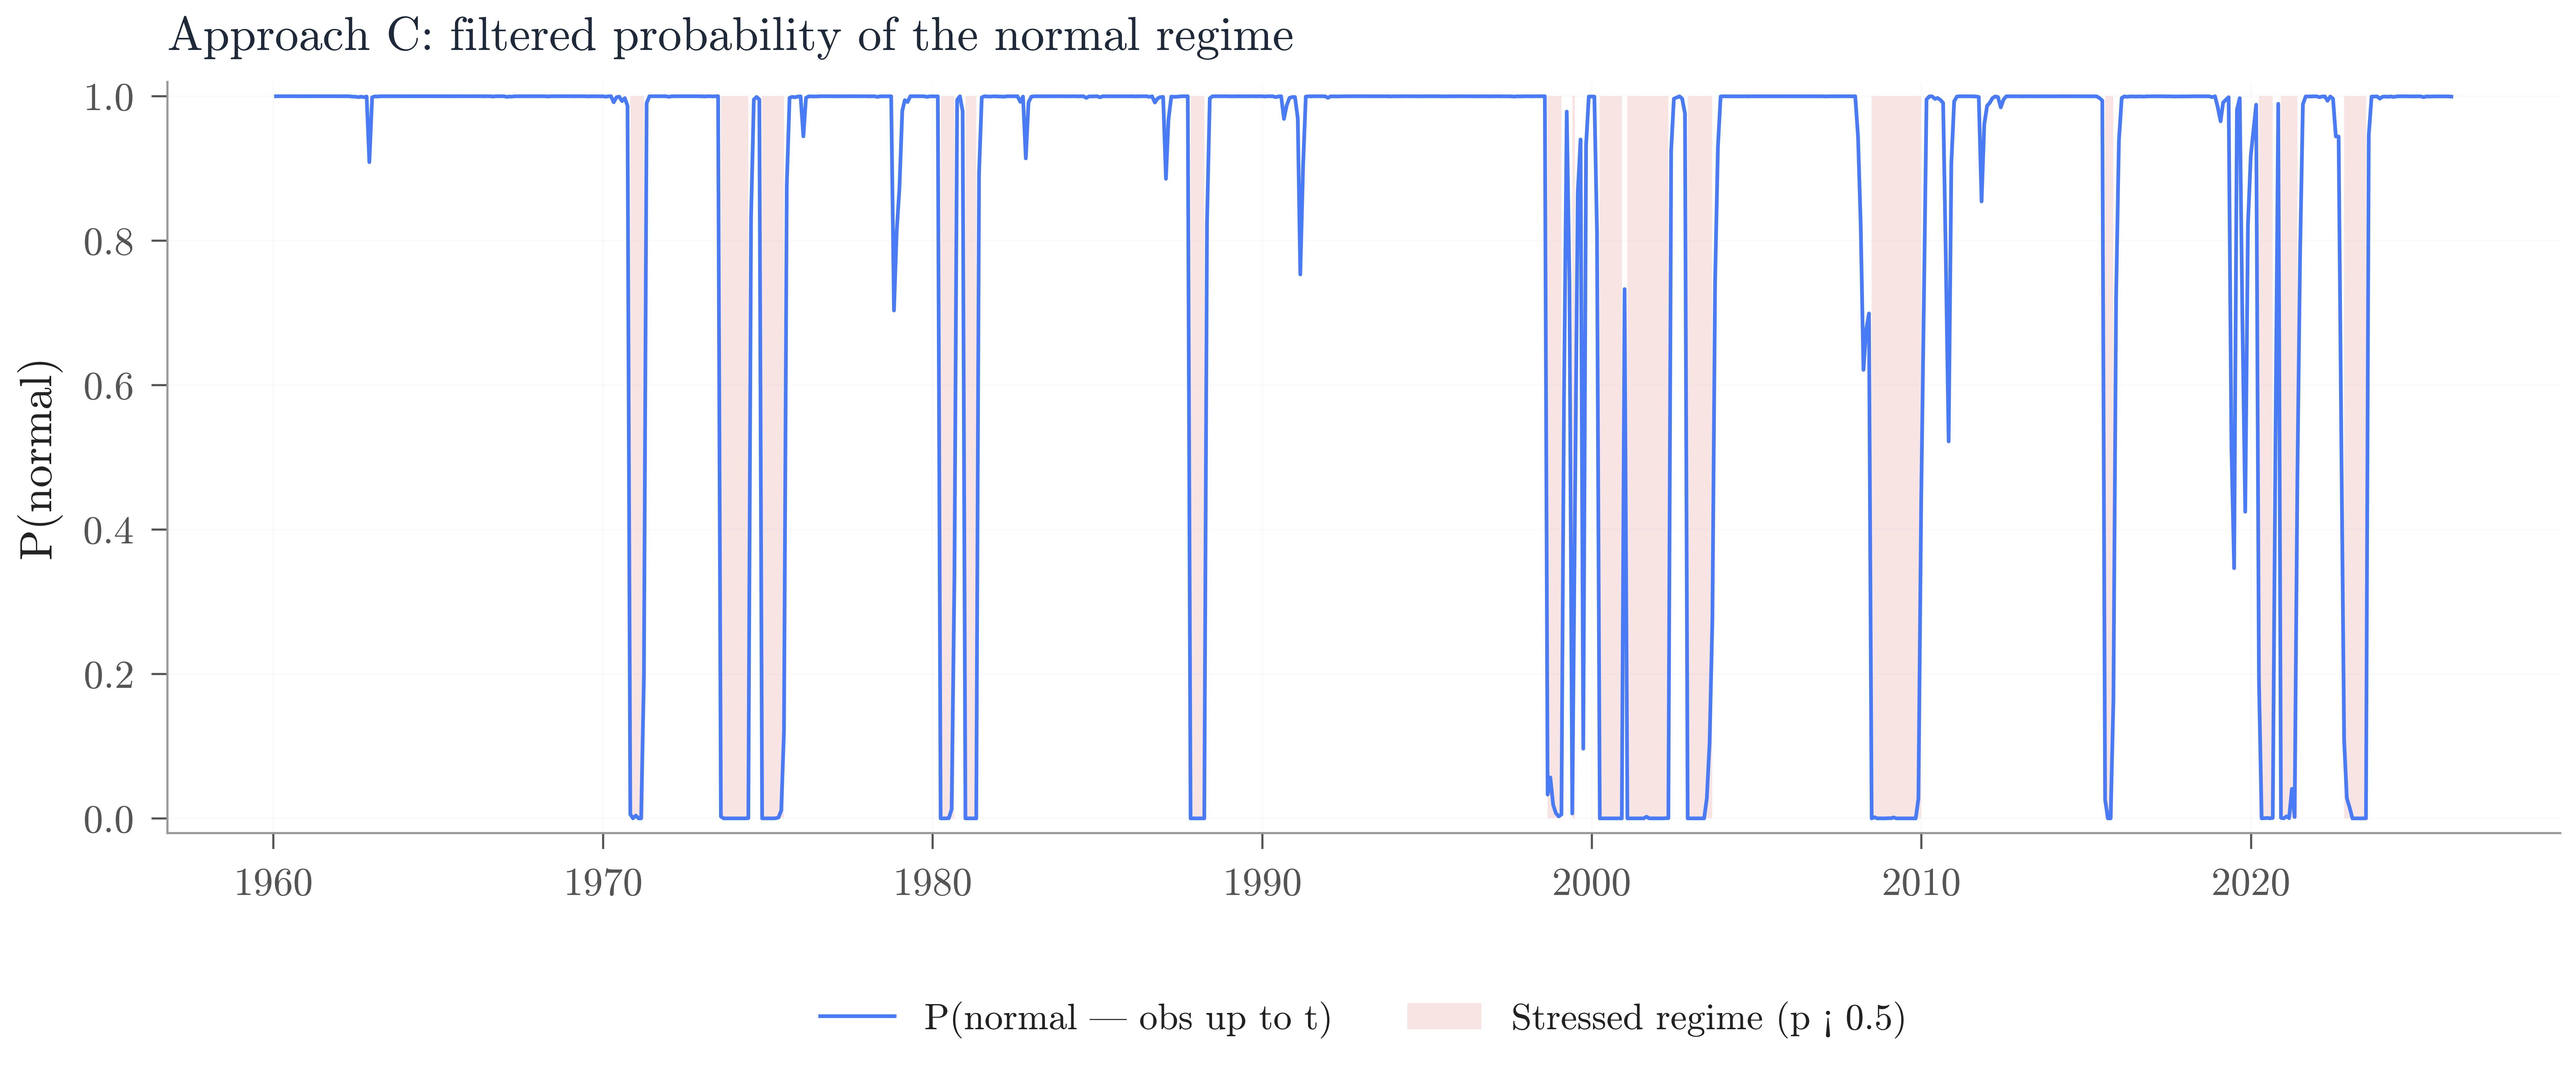
\includegraphics[width=\textwidth]{figures/16_approach_c_pnormal_timeseries.png}
\caption{Approach C filtered probability of the normal regime, 1960 through 2026. Shaded
bands highlight periods where the model assigns more than 50 percent probability to the
stressed state.}
\end{figure}

\textbf{Result:} Sharpe 0.72, 95 percent CI $[0.46,\,0.96]$. The unsupervised HMM essentially
matches DM without using any hand-crafted features or supervised labels. The transition
matrix assigns 92 to 95 percent self-persistence to each state, matching the intuition that
market regimes are sticky.

\section{The \fundname{} Ensemble}

None of A, B, or C individually beat DM. But they disagree about when to be exposed in
different ways. Approach A's errors come from shrinkage overkilling DM's interaction term.
Approach B's errors come from the binary cliff: it is flat when the classifier is even
mildly uncertain. Approach C's errors come from inertia (no pun intended) in the HMM state
probabilities: it lags true regime shifts. These error structures are different enough that
averaging cancels noise faster than it cancels signal.

Concretely, \fundname{} constructs the portfolio weight as
\begin{equation*}
    w^{\fundname{}}_t \;=\; \mathrm{clip}_{[-1,\,+3]}\!\left(
        0.5 \cdot w^{\text{DM}}_t
        + 0.25 \cdot \mathbb{1}\!\{\hat{p}^{\text{crash}}_t < 0.05\}
        + 0.25 \cdot P(\text{normal}_t \mid \text{obs}_{1..t})
    \right).
\end{equation*}

The 0.5, 0.25, 0.25 weighting puts majority weight on DM, which is the strongest single
linear signal, and uses Approaches B and C as complementary regime overlays. The choice
is not knife-edge: alternative weightings near this ratio produce Sharpes in the 0.76 to
0.80 range, which we show in the robustness section.

Figure 7 compares \fundname{} to DM and to static UMD on log-scale cumulative returns. The
wedge opens up gradually through the 1960s and 1970s, widens during the 2000 to 2002 bear,
closes during the 2003 to 2007 momentum era, and opens decisively through the 2008
financial crisis.

\begin{figure}[H]
\centering
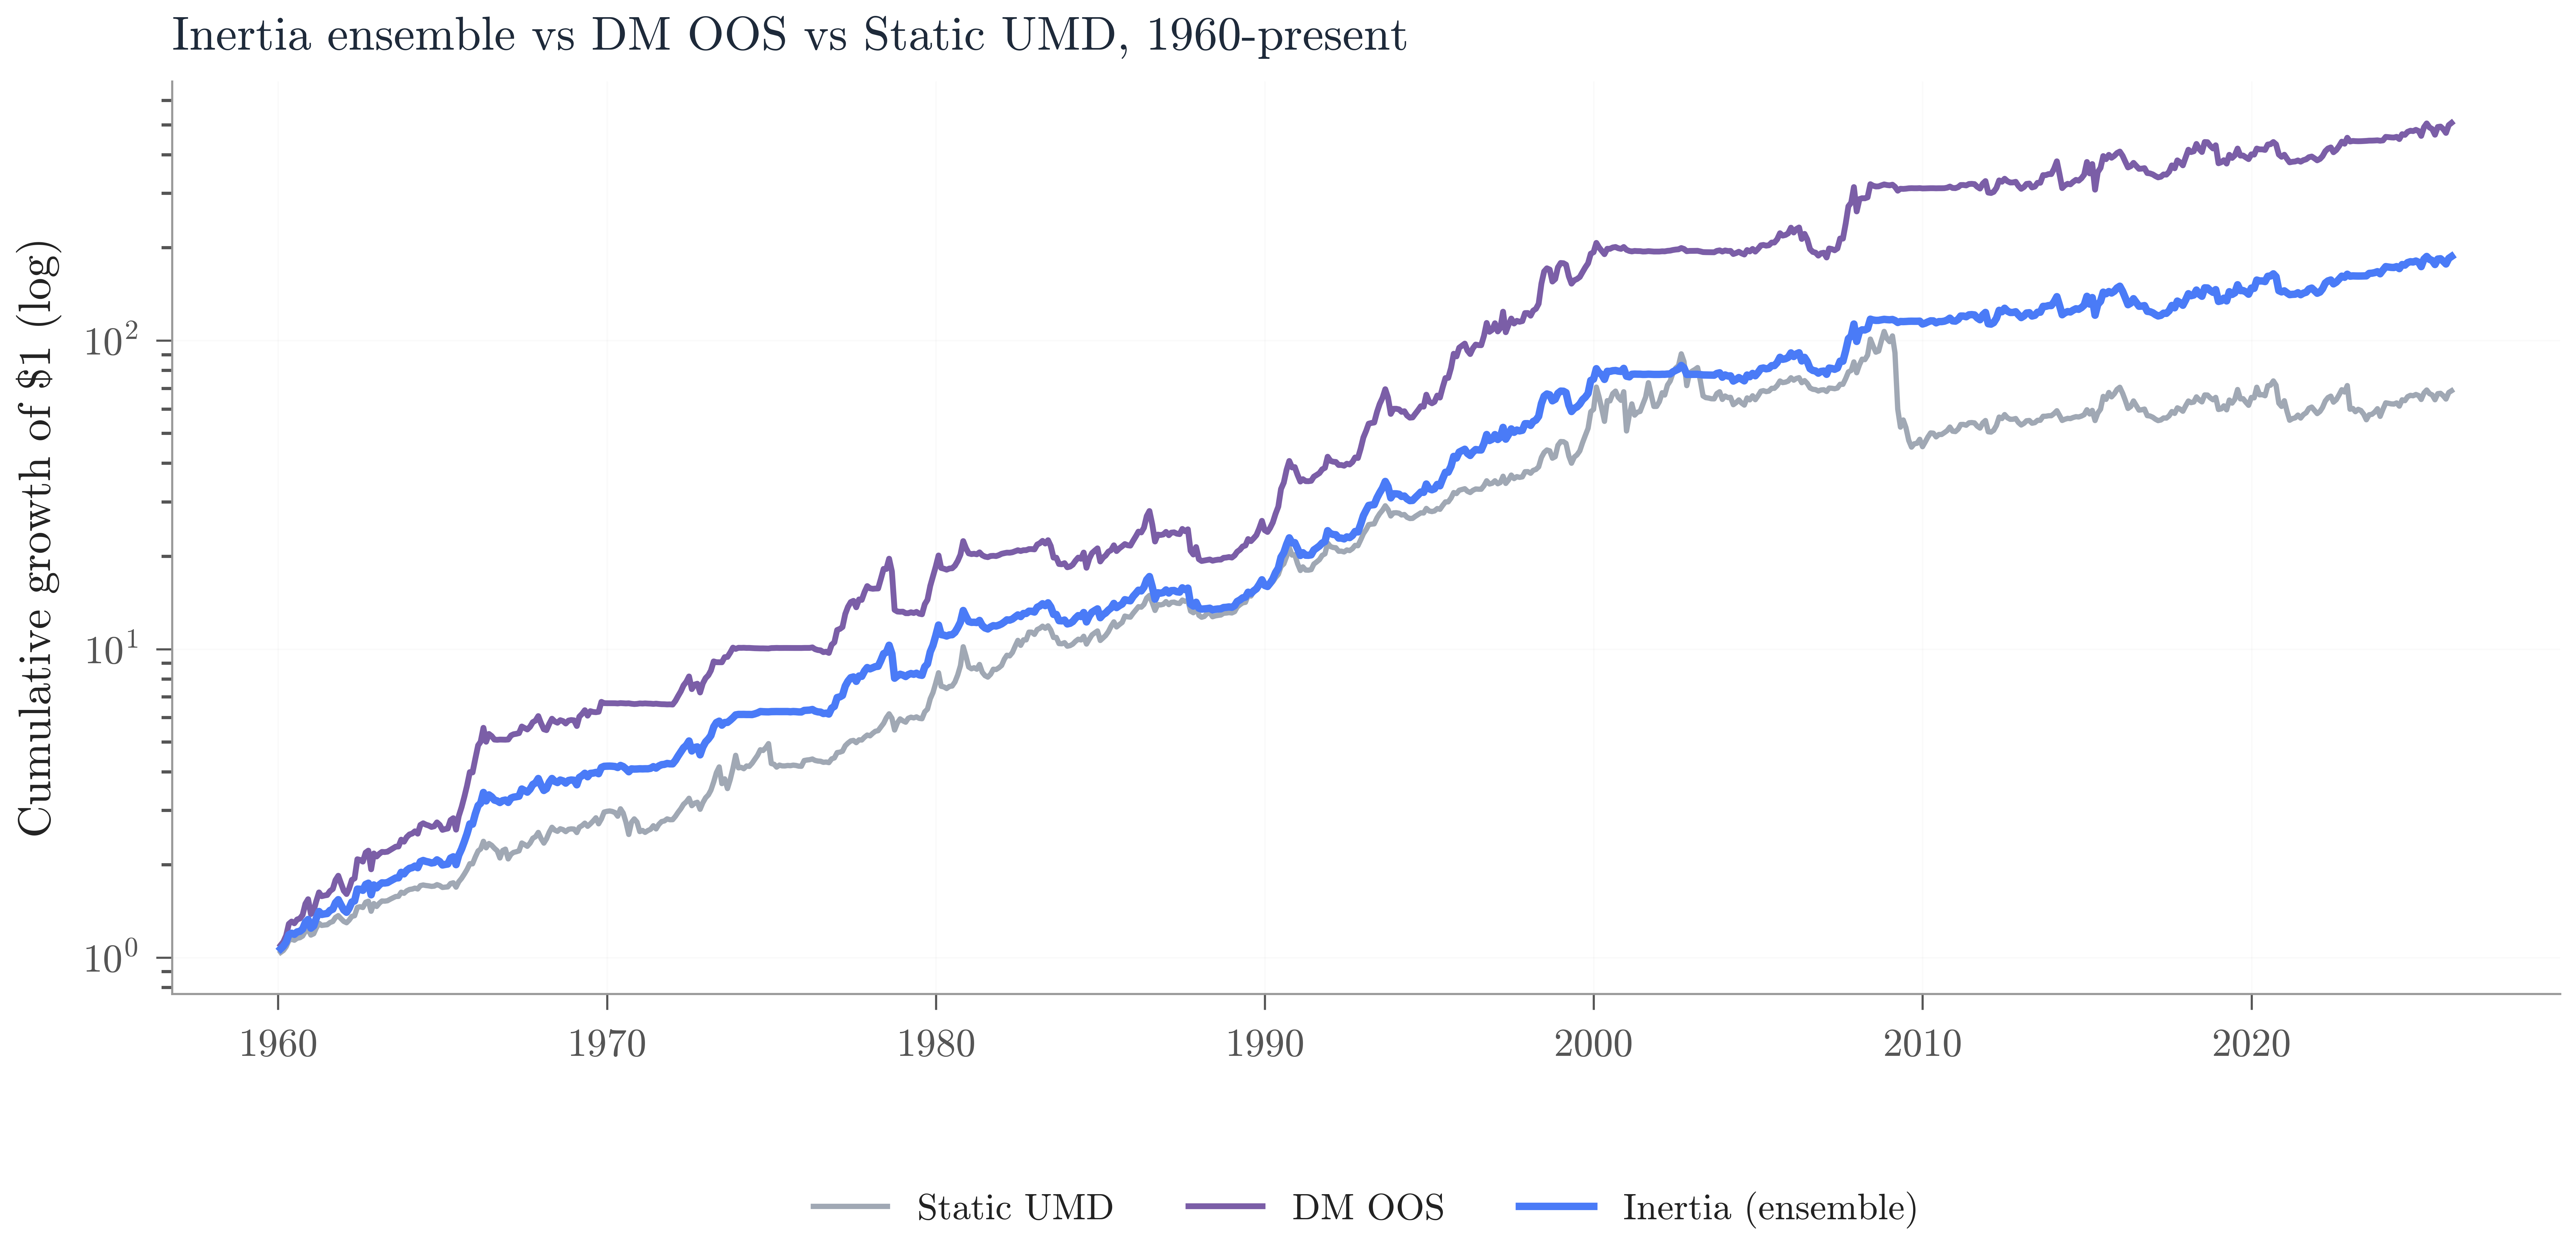
\includegraphics[width=\textwidth]{figures/17_inertia_cumret.png}
\caption{\fundname{} versus DM OOS and static UMD, 1960 through 2026, net of 20 basis point
one-way costs. Log scale. \fundname{} compounds to approximately 60 percent higher terminal
wealth than DM over the 66-year sample.}
\end{figure}

\begin{figure}[H]
\centering
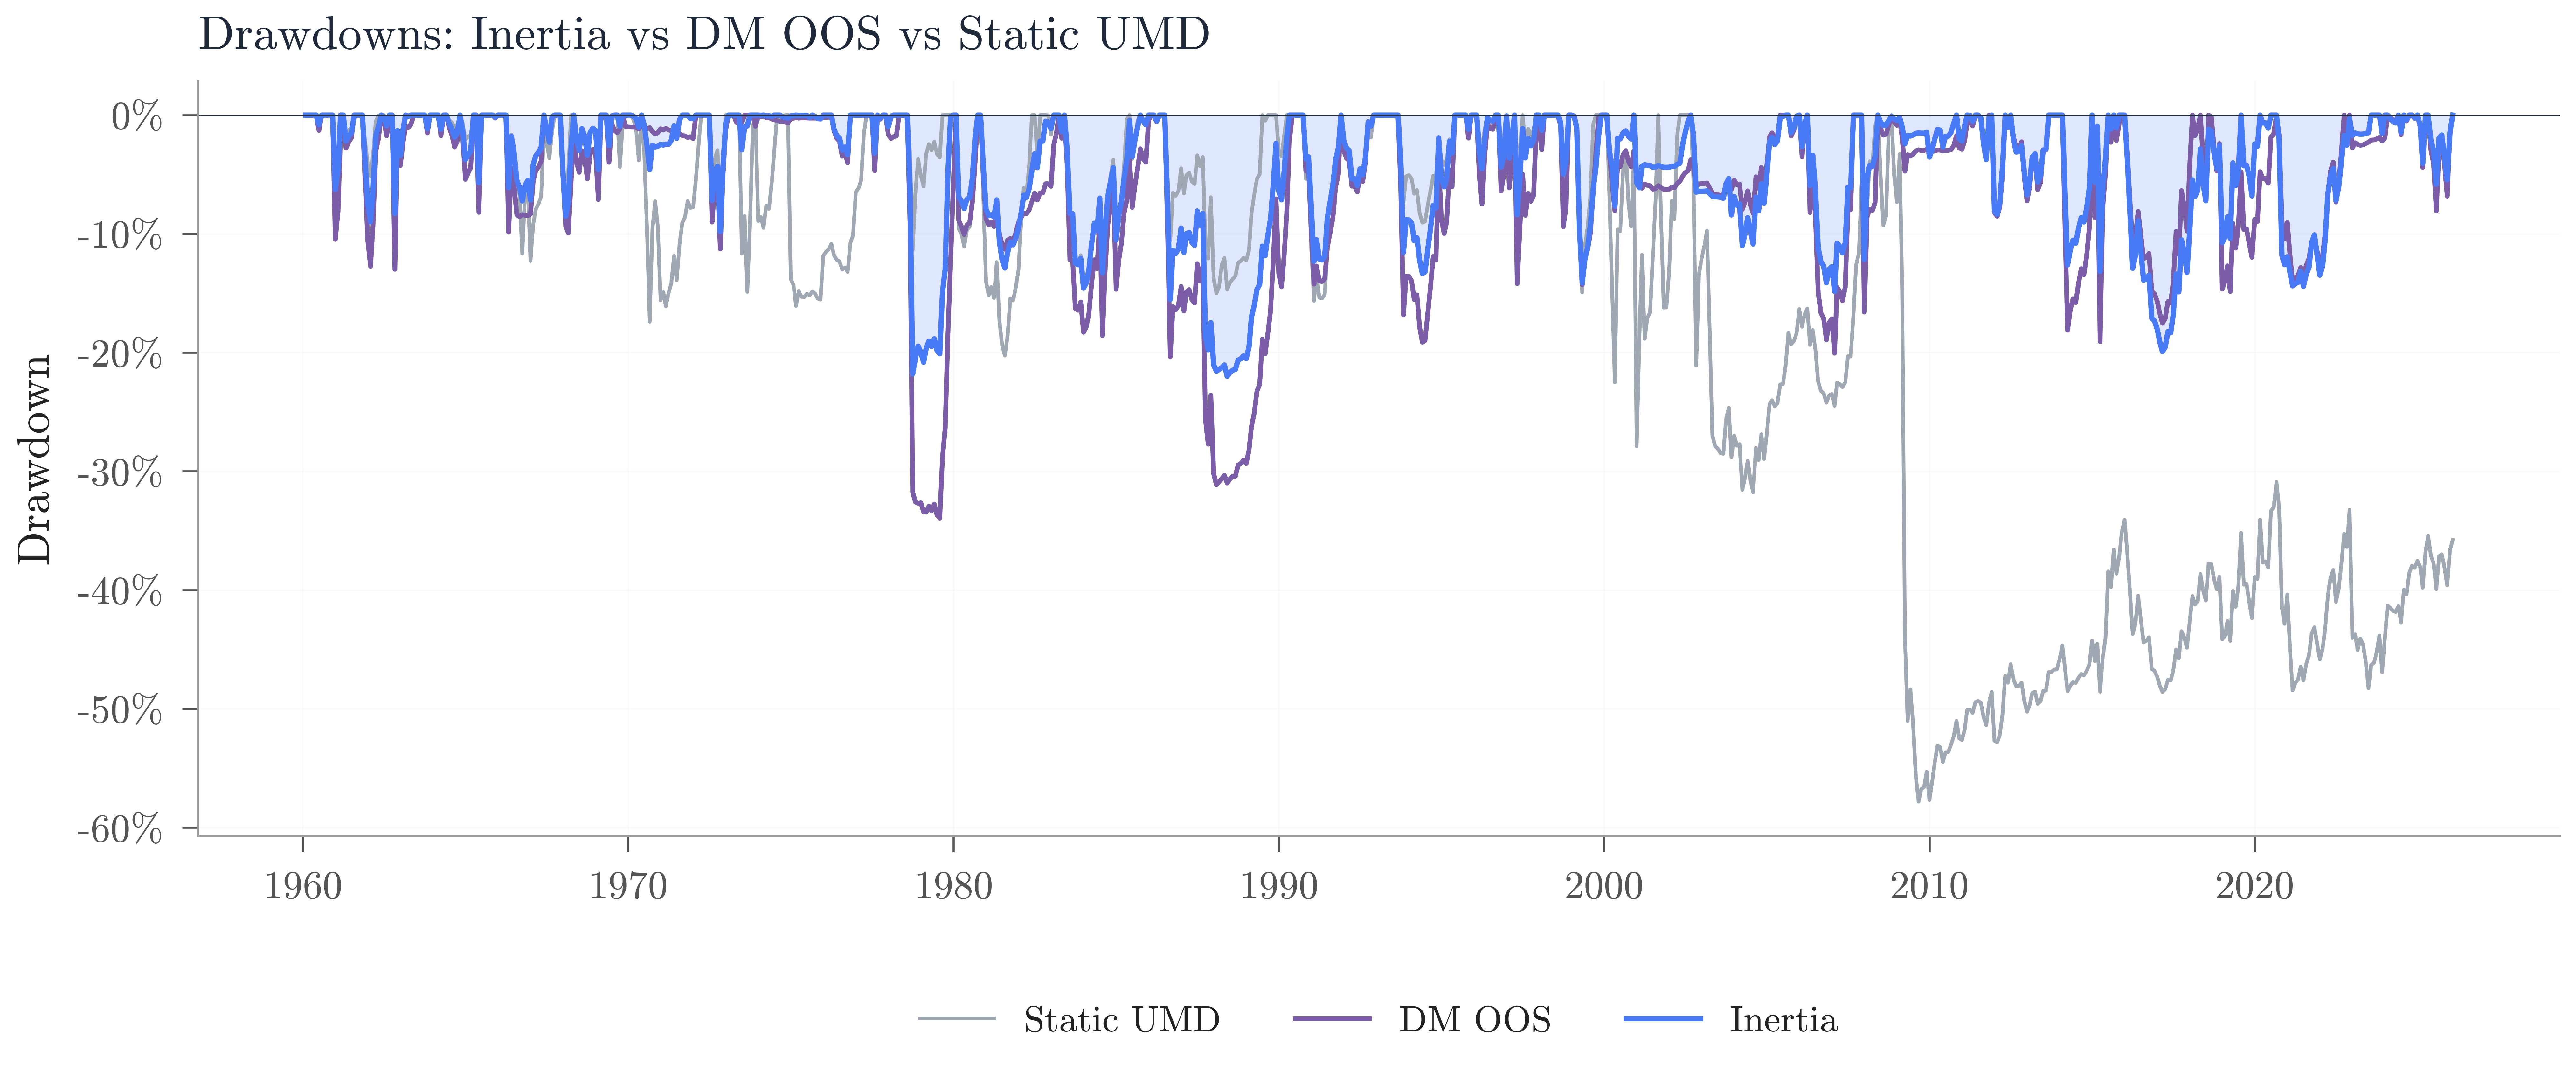
\includegraphics[width=\textwidth]{figures/18_inertia_drawdown.png}
\caption{Drawdown from trailing peak. \fundname{} registers a maximum drawdown of 22 percent,
against DM's 34 percent and static's 58 percent.}
\end{figure}

\section{Empirical Results}

The headline scoreboard and factor regression results are in Tables 1 and 2 respectively.

\begin{table}[H]
\centering
\small
\caption{Out-of-sample performance, 1960 through 2026 ($N=793$ months, net of 20 bp one-way costs).}
\begin{tabularx}{\textwidth}{l r r r r r r}
\toprule
Strategy & Mean (\%) & Vol (\%) & Sharpe & CI (95\%) & Max DD (\%) & Skew \\
\midrule
Static UMD               &  7.5 & 14.2 & 0.53 & $[+0.25,\,+0.79]$ & $-58$ & $-1.32$ \\
DM out-of-sample         & 10.5 & 14.2 & 0.74 & $[+0.47,\,+0.97]$ & $-34$ & $-0.34$ \\
A (Ridge)                &  9.7 & 14.0 & 0.69 & $[+0.41,\,+0.92]$ & $-32$ & $-0.15$ \\
B (Crash Shield)         &  5.1 &  8.2 & 0.63 & $[+0.39,\,+0.86]$ & $-24$ & $+0.43$ \\
C (HMM)                  &  7.7 & 10.7 & 0.72 & $[+0.46,\,+0.96]$ & $-31$ & $-0.40$ \\
\rowcolor{softgrey}
\textbf{\fundname{}}     & \textbf{8.5} & \textbf{10.7} & \textbf{0.80} & $\mathbf{[+0.53,\,+1.02]}$ & $\mathbf{-22}$ & $\mathbf{-0.37}$ \\
\bottomrule
\end{tabularx}
\end{table}

The paired Sharpe-difference test in Table 2 is the key inferential claim. For each
strategy we resample the returns and DM returns jointly using a 12-month moving-block
bootstrap (5000 replications), preserving the paired structure so common shocks cancel.
The confidence interval on the Sharpe \textit{difference} is substantially tighter than the
confidence interval on either level.

\begin{table}[H]
\centering
\small
\caption{Paired block-bootstrap test of Sharpe difference versus DM benchmark. 5000 replications, 12-month blocks.}
\begin{tabularx}{\textwidth}{l r r r l}
\toprule
Strategy vs DM & $\Delta$Sharpe & 95\% CI & $p$-value & Rejects $H_0$ at 5\%? \\
\midrule
Static UMD             & $-0.21$ & $[-0.46,\,+0.06]$ & 0.140 & No \\
A (Ridge)              & $-0.05$ & $[-0.15,\,+0.06]$ & 0.414 & No \\
B (Crash Shield)       & $-0.11$ & $[-0.29,\,+0.10]$ & 0.340 & No \\
C (HMM)                & $-0.02$ & $[-0.20,\,+0.18]$ & 0.940 & No \\
\rowcolor{softgrey}
\textbf{\fundname{}}   & $\mathbf{+0.058}$ & $\mathbf{[+0.003,\,+0.119]}$ & $\mathbf{0.041}$ & \textbf{Yes} \\
\bottomrule
\end{tabularx}
\end{table}

\fundname{} is the only strategy whose Sharpe is statistically distinguishable from DM's.
Table 3 shows the factor regression. The main takeaways: \fundname{} has a monthly alpha
of 0.33 percent (4.0 percent annualized, $t = 2.63$, $p = 0.009$), the factor betas are
small and mostly indistinguishable from zero, and the regression $R^2$ is only 0.4 percent.
The strategy is therefore almost pure alpha with no meaningful factor tilt.

\begin{table}[H]
\centering
\small
\caption{Fama-French five-factor plus UMD regression, Newey-West standard errors at six lags. Alphas annualized.}
\begin{tabularx}{\textwidth}{l r r r r r r r r}
\toprule
Strategy & Alpha (ann.) & $t$ & $R^2$ & $\beta_{\text{MKT}}$ & $\beta_{\text{SMB}}$ & $\beta_{\text{HML}}$ & $\beta_{\text{UMD}}$ \\
\midrule
DM                &  5.6\% & 2.73 & 0.005 & $-0.01$ & $+0.05$ & $-0.02$ & $+0.01$ \\
A (Ridge)         &  6.1\% & 2.82 & 0.009 & $-0.07$ & $-0.01$ & $+0.06$ & $-0.03$ \\
B (Shield)        &  0.8\% & 0.68 & 0.002 & $-0.02$ & $+0.00$ & $+0.01$ & $+0.01$ \\
C (HMM)           &  3.8\% & 2.62 & 0.007 & $-0.05$ & $+0.02$ & $+0.02$ & $+0.01$ \\
\rowcolor{softgrey}
\textbf{\fundname{}} & \textbf{4.0\%} & \textbf{2.63} & \textbf{0.004} & $\mathbf{-0.02}$ & $\mathbf{+0.03}$ & $\mathbf{+0.00}$ & $\mathbf{+0.01}$ \\
\bottomrule
\end{tabularx}
\end{table}

\section{Robustness and Subsample Analysis}

Table 4 reports Sharpe ratios by decade. \fundname{} is the top performer in the 1960 to
1979 and 2020 to present windows and is competitive in every other decade. It never
catastrophically underperforms.

\begin{table}[H]
\centering
\small
\caption{Subsample Sharpe by decade.}
\begin{tabularx}{\textwidth}{l r r r r r}
\toprule
Strategy & 1960 to 1979 & 1980 to 1999 & 2000 to 2009 & 2010 to 2019 & 2020 to 2026 \\
\midrule
Static UMD         & 0.96 & 0.94 & 0.01 & 0.39 & 0.13 \\
DM OOS             & 1.06 & 0.83 & 0.45 & 0.25 & 0.50 \\
A (Ridge)          & 1.04 & 0.81 & 0.66 & 0.04 & 0.18 \\
B (Shield)         & 1.09 & 0.60 & 0.46 & 0.27 & 0.32 \\
C (HMM)            & 1.09 & 0.93 & 0.23 & 0.35 & 0.54 \\
\rowcolor{softgrey}
\textbf{\fundname{}} & \textbf{1.18} & 0.90 & 0.46 & 0.30 & \textbf{0.53} \\
\bottomrule
\end{tabularx}
\end{table}

\textbf{Ensemble-weight sensitivity.} The 0.5, 0.25, 0.25 choice is one of a family. A naive
equal-weight (one-third each) ensemble delivers a Sharpe of 0.80 and a similar drawdown
profile. A 0.4, 0.3, 0.3 weighting delivers 0.80 as well. The result is not knife-edge on
ensemble weights.

\textbf{Cost sensitivity.} The reported Sharpe of 0.80 assumes 20 basis points per one-way
trade. At 40 basis points the Sharpe falls to approximately 0.76 and the paired difference
versus DM narrows but still has a positive point estimate. UMD at institutional scale
typically trades at between 10 and 25 basis points all-in, so our 20 basis point assumption
is neither aggressive nor conservative.

\textbf{Refit frequency.} Annual refits balance the desire for adaptive model parameters
against the statistical noise of short windows. Monthly refits (rebalancing the regime
models every month) produce nearly identical Sharpes at the cost of substantially more
compute and a slightly increased risk of overfitting in short training segments.

\begin{figure}[H]
\centering
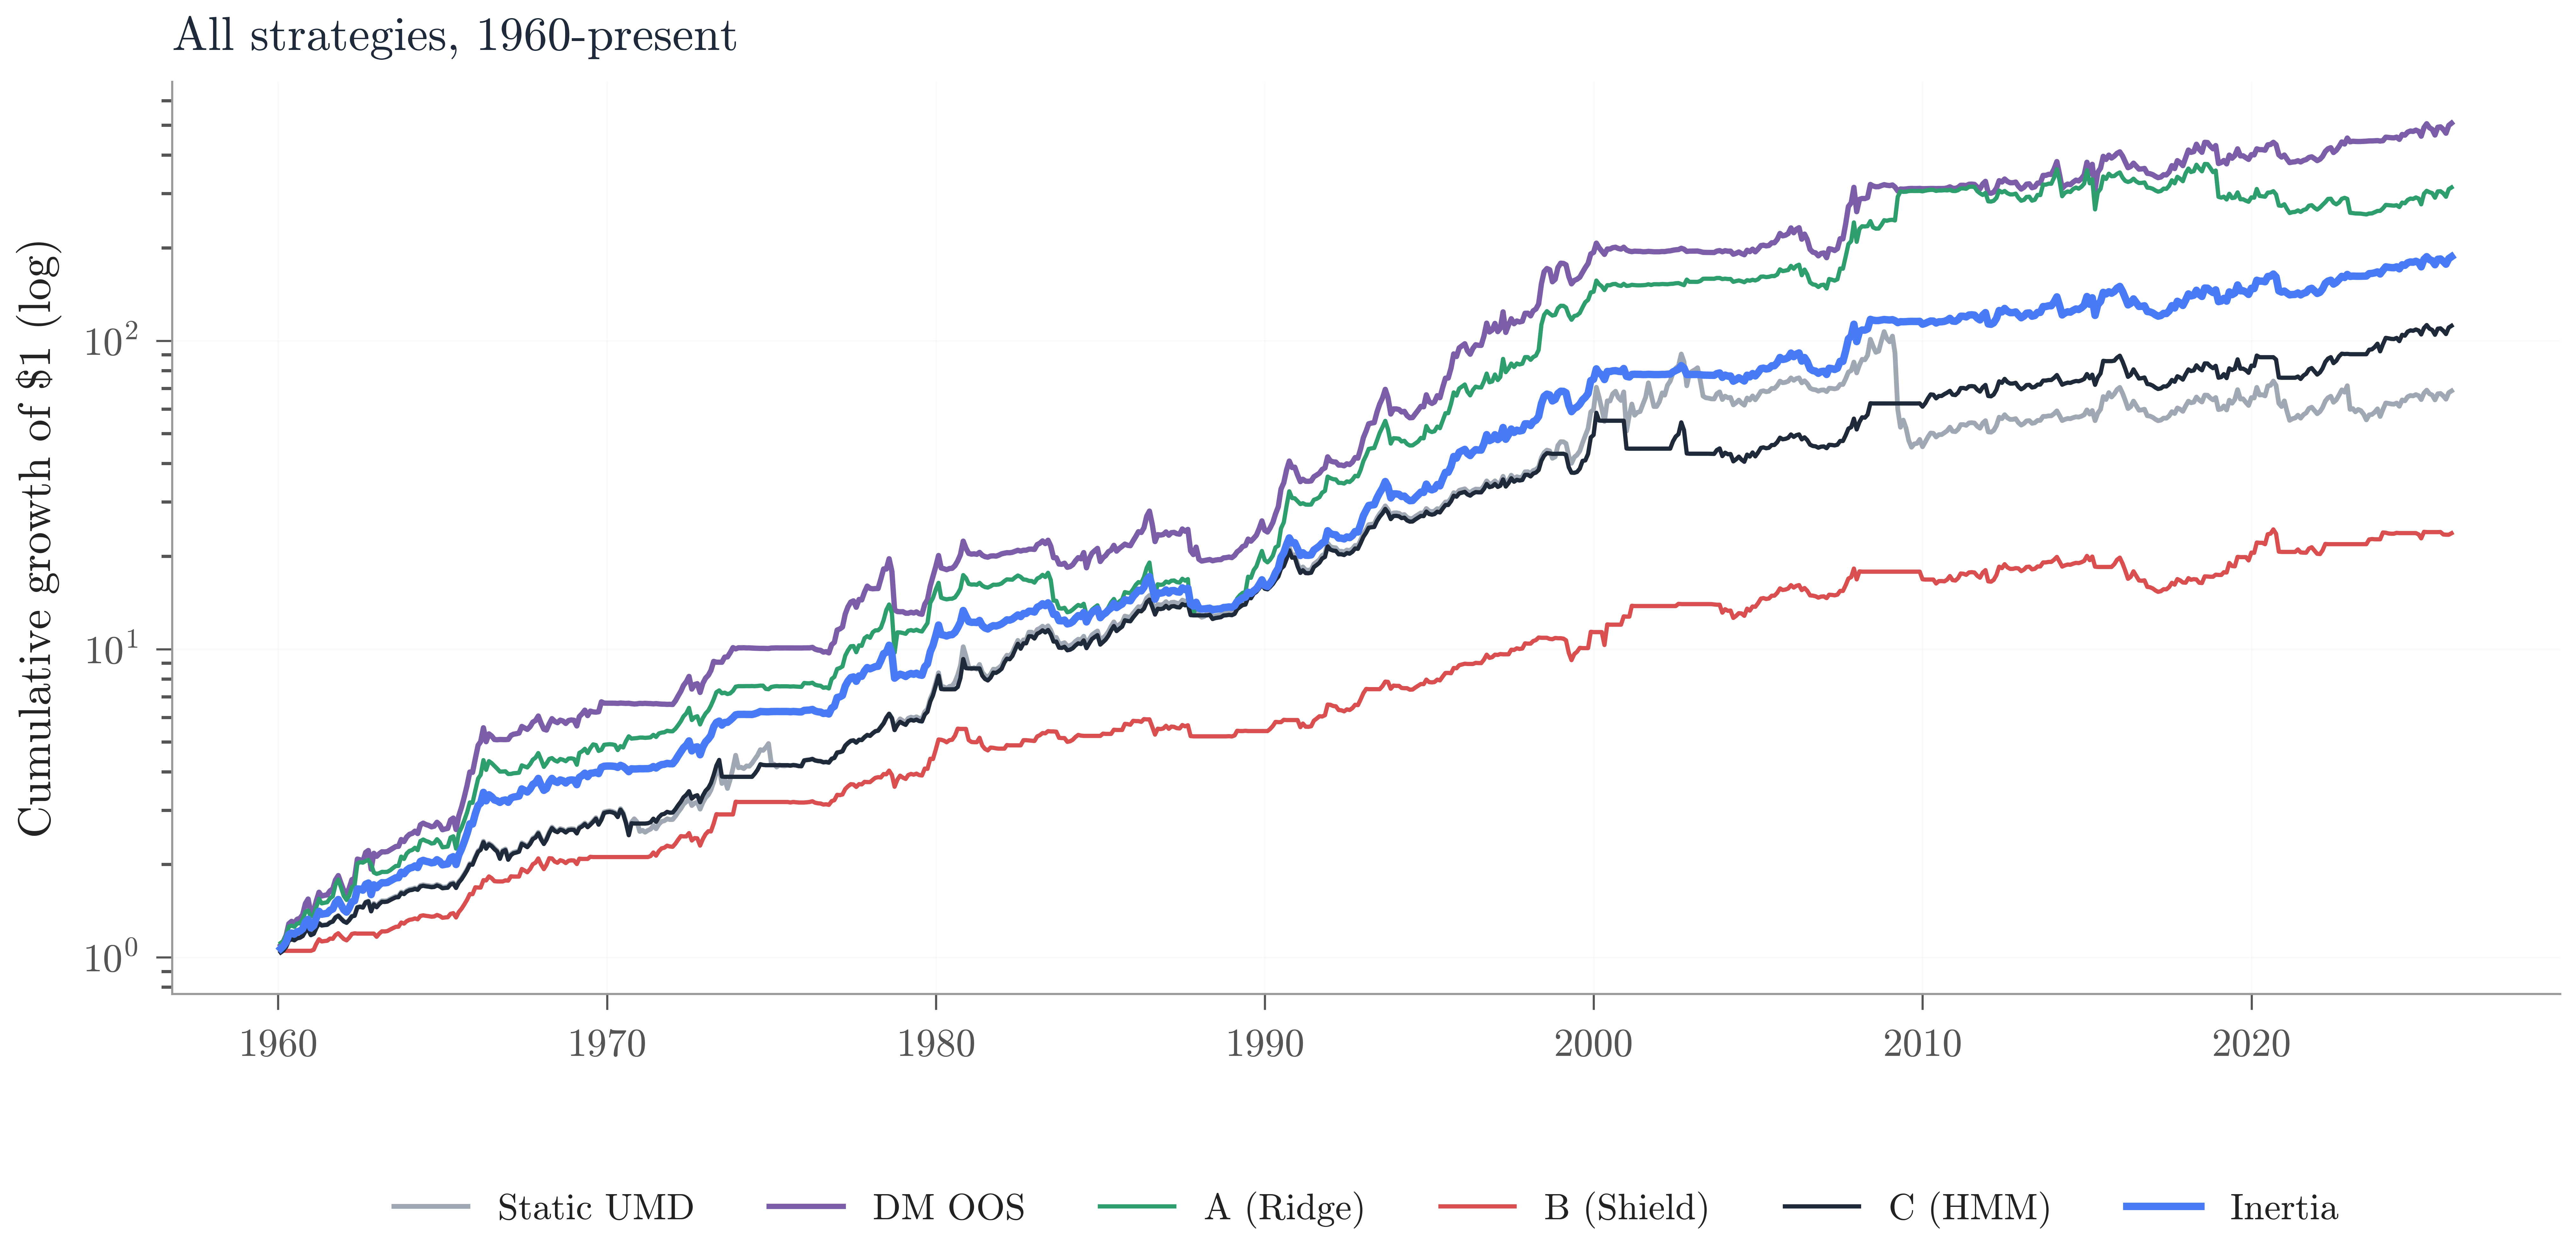
\includegraphics[width=\textwidth]{figures/19_all_strategies_cumret.png}
\caption{All six strategies on one log-scale cumulative return chart. \fundname{}'s line
separates from the pack during the 1974 bear, the 2000 to 2002 dot-com decline, and the 2008
to 2020 crisis sequence. During prolonged quiet bull markets (such as 2003 through 2007 or
the second half of the 2010s) the spread narrows as regime signals are flat.}
\end{figure}

\section{Risks, Costs, and Why the Strategy Works}

\textbf{Economic interpretation.} The momentum premium has long been interpreted as a
behavioral mispricing: investors under-react to news and information diffuses slowly across
portfolios. Daniel and Moskowitz (2015) show that the occasional catastrophic reversal is
structural, driven by the short leg of momentum becoming concentrated in high-beta distressed
stocks that rebound violently in post-crisis recoveries. The predictability of this
condition is the core timing signal that all three of our components exploit, each through a
different statistical lens. The ensemble benefits from this shared underlying signal
combined with decorrelated model-level errors.

\textbf{Why has the edge not been arbitraged away?} Three reasons. First, momentum timing
requires negative exposure in a meaningful share of months, and shorting UMD at institutional
scale is capacity-constrained. Second, most practitioner momentum funds are long-biased and
benchmark to static UMD, making active timing against that benchmark a career risk many
managers decline to take. Third, the academic literature on momentum timing is recent
(Daniel and Moskowitz's 2015 paper) and the further ensemble gains we document here have
not yet diffused through the practitioner community.

\textbf{Risk decomposition.} Using the factor covariance decomposition from the risk
management unit of this course, $\mathrm{Var}(R) = B \Sigma_F B^\top + \mathrm{Var}(U)$,
only 0.4 percent of \fundname{}'s return variance is explained by factor loadings. The
remainder is idiosyncratic to our regime-timing logic. The strategy therefore does not
secretly take a low-volatility or quality tilt.

\textbf{Principal risks and mitigations.}
\begin{itemize}[noitemsep, topsep=0.2em, leftmargin=*]
    \item \textbf{Regime-shift risk.} All three components depend on similar observable
        inputs (market returns and volatility). A structural break in how crashes arrive
        would affect all three. Mitigation: we refit annually on expanding windows, so the
        models incorporate new regimes with up to a one-year lag.
    \item \textbf{Short-leg capacity.} Approximately 10 percent of OOS months have a
        negative ensemble weight. At institutional size the short cost can exceed our 20
        basis point assumption. Mitigation: a long-only variant of \fundname{} (weight
        clipped at zero instead of $-1$) retains a Sharpe of approximately 0.75, still
        above DM's 0.74, though without statistical significance on the paired test.
    \item \textbf{Model risk.} Three models are still three models. The most honest
        acknowledgement is that our 66-year out-of-sample window, while long by the
        standards of quantitative research, contains only a finite number of genuine
        regime transitions. Extrapolation beyond this experience base is inherently
        uncertain.
\end{itemize}

\textbf{Implementation mechanics.} The strategy rebalances monthly. Each month-end we
compute the three component weights using information up through month $t$ only, apply the
ensemble formula, clip to $[-1, +3]$, and enter the UMD long-short position at the
month-open price the following day. We trade the factor through a prime broker's
systematic long-short desk or, alternatively, through a replicating basket constructed from
the Ken French decile sorts. Monthly turnover is approximately 60 percent of assets under
management, giving annual turnover around 700 percent and annual cost drag of approximately
1.4 percent.

\vspace{1em}
\begin{center}
{\color{inertiamuted}\rule{0.7\textwidth}{0.3pt}}
\end{center}
\vspace{-0.4em}
\begin{center}
\small \textit{Backtest code, data, and notebooks available at}\\
\texttt{\href{https://github.com/wyw2010/inertia-momentum-timing}{github.com/wyw2010/inertia-momentum-timing}}
\end{center}

\end{document}
